\documentclass[10pt,a4paper]{article}
\usepackage[margin=2cm]{geometry}
\usepackage{amsmath,amssymb,booktabs,graphicx,caption,subcaption,xcolor,float,hyperref,tikz}
\usetikzlibrary{arrows.meta,positioning,calc}
\hypersetup{colorlinks=true,linkcolor=blue!50!black,urlcolor=blue!50!black}
\captionsetup{font=small,labelfont=bf}
\newcounter{diagram}
\newcommand{\diagramcaption}[1]{\refstepcounter{diagram}\par\smallskip\noindent{\small\textbf{Diagram~\thediagram.} #1}}
\title{\vspace{-1.2cm}\textbf{A swarm that owns a proof can still lose it, less often without rounds}\\[2pt]
\large Simulation 2 (asynchronous activation), setup \texttt{task003-symmetric}}
\author{LLM-free simulator; report of 14 October 2026; runs of 9 October 2026\\
\small Mirrors the Simulation 1 report on \texttt{task003-symmetric} of the same date, section by section.}
\date{}
\begin{document}
\maketitle
\vspace{-1cm}

\paragraph{How the simulator works.} The world, \texttt{task\_003}, has three candidate
allocations; A0 is the correct one. Each of 24 agents is given one true fact about it and reasons as
an exact Bayesian: its \emph{belief} is the exact probability of A0, A1 and A2 given the facts it
currently remembers. There are no rounds. Each agent acts at random times, on average once per time
unit: it reads $q$ posts drawn at random from the 48 most recent posts on a shared \emph{board}
(never its own), adds their facts to its memory, recomputes its belief, \emph{votes} by probability
matching (a vote drawn from its belief) and posts one remembered fact that supports its vote, or
nothing if none does. Every remembered fact is forgotten after a random lifetime (on average a
fraction $\rho$ survives one time unit; reading it again renews it). A \emph{controller} with a
target, A0 (truth) or A2 (false), acts at random times at rate $\lambda_c$ until $t = 30$: it reads
$q_c$ recent agent posts and, unless the \emph{vote gate} (at least 75\% of them from agents voting
for its target) or the \emph{proof stop} (its target already proved) silences it, posts the one fact
from its pool that best supports its target, at most 30 messages per episode. Agents continue alone
until $t = 40$. Every episode is run three times with the same random draws: without a controller,
with the truth controller and with the false controller.

\paragraph{Summary.} The 24 agents together hold a proof of allocation A0 (the truth).
Simulation 2 removes the day/night rounds of Simulation 1: agents and the controller act at
random times, remembered facts fade continuously, and the shared board fades too.
(i)~\textbf{Whether the false controller wins depends on memory}: when agents forget it pulls
part of the swarm to A2; with full memory every agent ends up proving A0. (ii)~\textbf{The false
controller is weaker than in Simulation 1}, in beliefs ($0.13$ against $0.22$) and in votes ($0.11$
against $0.22$); the truth controller is unchanged. (iii)~How fast the controller acts matters
little for where the swarm ends up, but \textbf{fast controllers overshoot and then relax}.
(iv)~As in Simulation 1, help with the truth \textbf{replaces the agents' own proofs}.
(v)~Measured by the swarm's \emph{collective decision}, \textbf{overturning the proof has increasing
returns}: concentrating control in some runs beats every tested setting. Effects persist for ten
time units after the controller stops. \textbf{Correction to the 9 and 12 October reports}: in
votes, the silent swarm holds A0 as firmly as in Simulation 1 (85\% at $q = 6$); the lower belief
measured earlier comes partly from when beliefs are measured (Section~2).

\section{Setup}

\begin{center}
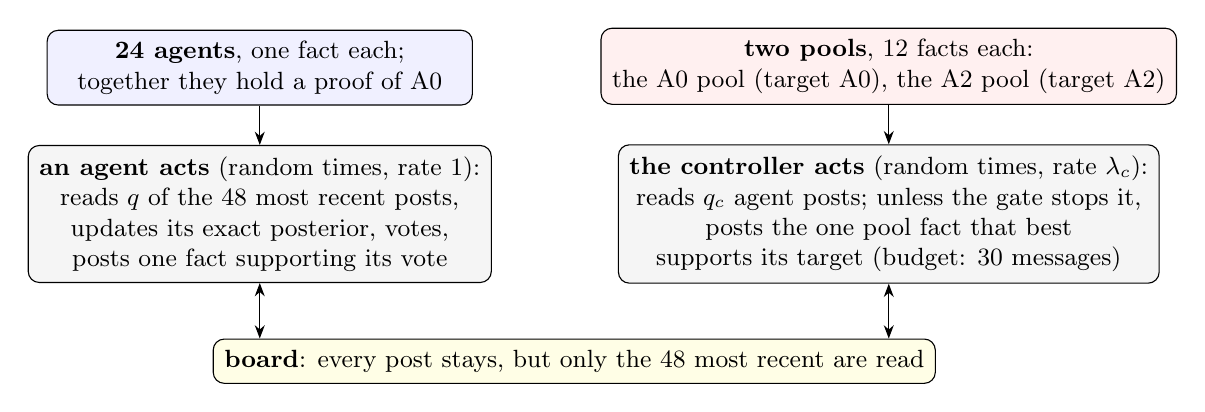
\begin{tikzpicture}[font=\small, box/.style={draw, rounded corners, align=center, inner sep=4pt}]
  \node[box, fill=gray!8, minimum width=5.4cm] (agent) {\textbf{an agent acts} (random times, rate 1):\\
     reads $q$ of the 48 most recent posts,\\ updates its exact posterior, votes,\\ posts one fact supporting its vote};
  \node[box, fill=gray!8, right=1.6cm of agent, minimum width=5.4cm] (ctrl) {\textbf{the controller acts} (random times, rate $\lambda_c$):\\
     reads $q_c$ agent posts; unless the gate stops it,\\ posts the one pool fact that best\\ supports its target (budget: 30 messages)};
  \node[box, fill=blue!6, above=0.5cm of agent, minimum width=5.4cm] (agents) {\textbf{24 agents}, one fact each;\\
     together they hold a proof of A0};
  \node[box, fill=red!6, above=0.5cm of ctrl, minimum width=5.4cm] (pool) {\textbf{two pools}, 12 facts each:\\
     the A0 pool (target A0), the A2 pool (target A2)};
  \coordinate (mid) at ($(agent.south)!0.5!(ctrl.south)$);
  \node[box, fill=yellow!10, anchor=north, minimum width=8cm] (board) at ($(mid)+(0,-0.7)$) {\textbf{board}: every post stays, but only the 48 most recent are read};
  \draw[-{Stealth}] (agents) -- (agent);
  \draw[-{Stealth}] (pool) -- (ctrl);
  \draw[{Stealth}-{Stealth}] (agent.south) -- (agent.south |- board.north);
  \draw[{Stealth}-{Stealth}] (ctrl.south) -- (ctrl.south |- board.north);
\end{tikzpicture}
\diagramcaption{Simulation 2. There are no rounds. Each remembered fact is forgotten after a
random lifetime (on average a fraction $\rho$ survives one time unit) and comes back if read
again. The controller acts for $0 \le t < 30$; agents continue alone until $t = 40$.}
\end{center}

\noindent The two pools share no fact, contain no decisive fact and cannot prove their target.
Agents are exact Bayesian reasoners. An agent's vote is drawn from its posterior
(probability matching). The \emph{vote gate} keeps the controller silent when at least 75\%
of the posts it read come from agents who voted for its target; the \emph{proof stop} keeps
it silent when what it read already proves its target. The grid: posts read
$q \in \{3,6,12\}$, $q_c \in \{3,6,12,24\}$, memory $\rho \in \{0.75, 1\}$, controller rate
$\lambda_c \in \{0.5,1,2,4,8\}$ actions per time unit, gate on/off, proof stop on/off;
1{,}000 episodes per setting. Control is measured by the \emph{gain}
\begin{equation}\label{eq:gain}
G(t) = \frac{1}{E}\sum_{e=1}^{E}\Bigl[m_{\text{target}}(t)^{\text{ctrl}}(e) - m_{\text{target}}(t)^{\text{silent}}(e)\Bigr],
\end{equation}
where $m_k(t)$ is the agents' mean belief in allocation $k$ and each episode $e$ uses the same
random draws with and without the controller. (Simulation 1 measures the gain in the share of
\emph{votes}; Table~\ref{tab:gain} gives both, and Figure~\ref{fig:votes} shows the vote shares of both
simulations on the same scale.) Unless stated otherwise: $q = 6$, $q_c = 12$, $\lambda_c = 1$,
gate on, proof stop on.

\section{Main result: the false controller can pull the swarm off its proof only when agents forget}

\begin{figure}[H]
\centering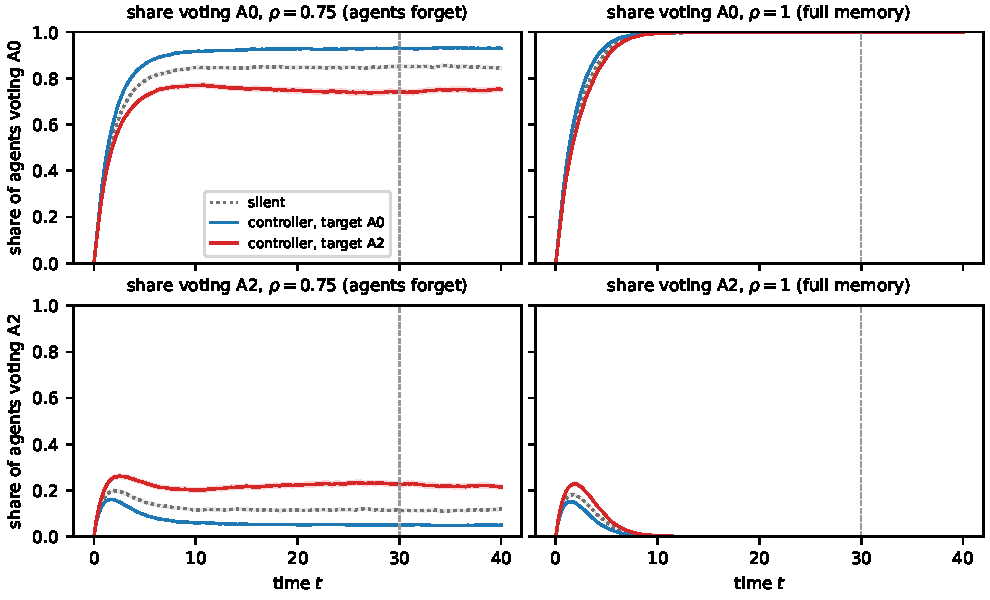
\includegraphics[width=0.84\linewidth]{figures/fig_votes_time.pdf}
\caption{Share of the 24 agents voting A0 (top) and A2 (bottom) over time, without a controller
(dotted grey), with the controller targeting A0 (blue) and with the one targeting A2 (red);
$\rho = 0.75$ (left) and $\rho = 1$ (right). Agents who have not acted yet have no vote, so the
shares start at 0 (all agents have voted by $t \approx 5$). The controller stops at $t = 30$
(dashed). Bands: 95\% intervals. $q = 6$, $q_c = 12$, $\lambda_c = 1$, gate on.}
\label{fig:votes}
\end{figure}

\begin{itemize}\itemsep1pt
\item \textbf{Without a controller the swarm backs the truth}: at $t = 30$, 85\% vote A0 and 12\% A2
  when agents forget; with full memory every agent votes A0 from $t \approx 10$.
\item \textbf{When agents forget, the false controller pulls part of the swarm away}: the A2 share
  doubles (0.23 against 0.12) and the A0 share falls to 0.74; the truth controller raises A0 to 0.93.
\item \textbf{With full memory the false controller wins only briefly}: an early bump in A2 (0.23
  at $t \approx 2$, against 0.18 silent), then every agent votes A0.
\end{itemize}

\paragraph{Without a controller, compared with Simulation 1.} In votes the silent swarm is as firm as
in Simulation 1: at $t = 30$, 85\% vote A0 at $q = 6$ (Simulation 1: 85\%) and 94\% at $q = 12$
(94\%). Measured as the agents' belief at a fixed moment it looks weaker ($m_{\text{A0}} = 0.72$ against
0.84 at $q = 6$; confirmed with fresh random draws), and fewer agents hold a complete proof (12\%
against 28\%). Part of this gap is timing: an agent votes right after reading, with a fresh memory,
and keeps forgetting until it acts again, so a snapshot at a fixed time catches faded memories; in
Simulation 1 the day-end snapshot comes before dawn's forgetting. We have not separated how much of
the proof gap is timing and how much is a real difference. The 9 October report read the belief gap
as ``the proof is held less firmly''; in the collective vote it is not.

\begin{table}[H]
\centering\small
\caption{Gain at $t = 30$, $\rho = 0.75$, $q_c = 12$, $\lambda_c = 1$, gate on, for $q = 3 / 6 / 12$: in
mean belief, Eq.~(\ref{eq:gain}), and in the share of votes for the target (the measure of
Simulation 1). Simulation 1: one fact per night, probability matching, same $q$, $q_c$. With full memory
every gain is 0.}
\label{tab:gain}
\begin{tabular}{lccc}
\toprule
controller & Simulation 2, belief & Simulation 2, votes & Simulation 1, votes \\
\midrule
truth (A0) & 0.12 / 0.08 / 0.04 & 0.14 / 0.08 / 0.04 & 0.17 / 0.08 / 0.01 \\
false (A2) & 0.20 / 0.13 / 0.09 & 0.24 / 0.11 / 0.04 & 0.41 / 0.22 / 0.06 \\
\bottomrule
\end{tabular}
\end{table}

\begin{figure}[H]
\centering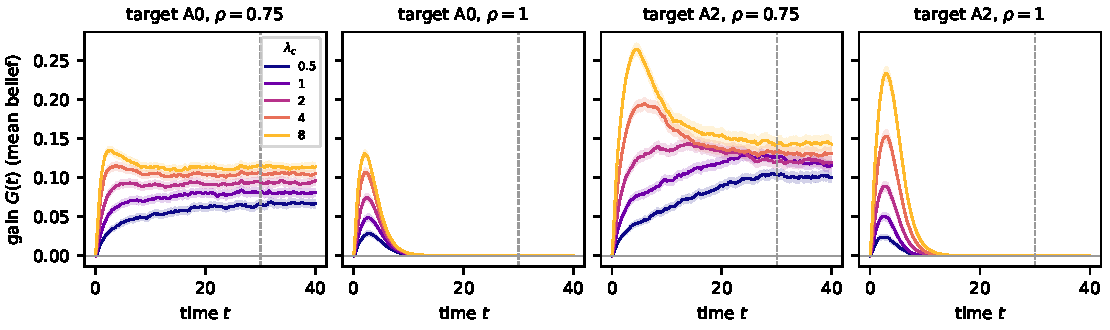
\includegraphics[width=0.98\linewidth]{figures/fig_gain_time.pdf}
\caption{Gain over time, Eq.~(\ref{eq:gain}), one line per controller rate $\lambda_c$; gate on.
The controller stops at $t = 30$ (dashed). Bands: 95\% intervals.}
\label{fig:gaintime}
\end{figure}

\begin{figure}[H]
\centering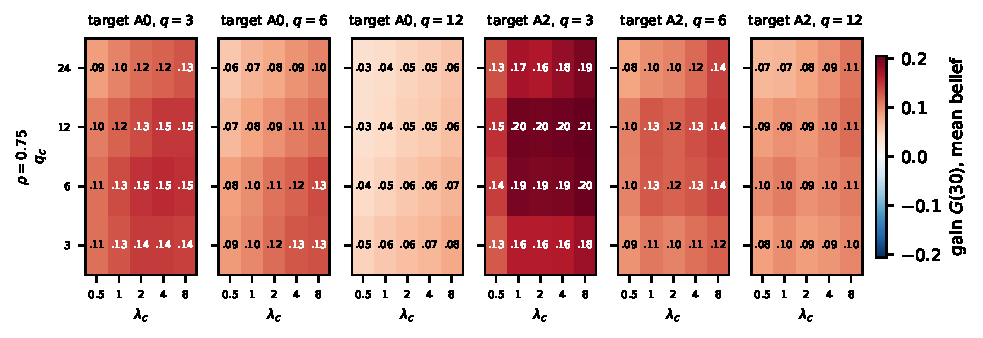
\includegraphics[width=0.98\linewidth]{figures/fig_phase_gain.pdf}
\caption{Gain $G(30)$ over the controller rate $\lambda_c$ (x) and the posts it reads $q_c$ (y), for
each target and every $q$ (columns), $\rho = 0.75$; gate on. With full memory every gain is 0.
Grey number: the 95\% interval includes 0.}
\label{fig:phase}
\end{figure}

\begin{itemize}\itemsep1pt
\item \textbf{The false controller is weaker than in Simulation 1}, in beliefs ($0.13$ against
  $0.22$; confirmed with fresh draws) and in votes ($0.11$ against $0.22$). The truth controller is
  unchanged ($0.08$ in both).
\item \textbf{Reading more defends the proof}: the false controller's gain falls from $0.20$ at
  $q = 3$ to $0.09$ at $q = 12$ (Table~\ref{tab:gain}, Figure~\ref{fig:phase}); agents who read more
  meet more pieces of the proof.
\item \textbf{The effect persists}: ten time units after the controller stops, the gain has
  changed by at most $0.021$ in every setting, less than one agent's worth of belief
  ($1/24 \approx 0.042$); confirmed with fresh draws. With full memory every gain is 0 by $t = 30$
  (Figure~\ref{fig:gaintime}, right panels).
\end{itemize}

\section{The controller's strength, the vote gate and the proof stop}\label{sec:strength}

\subsection{Strength: the controller's rate}

\begin{figure}[H]
\centering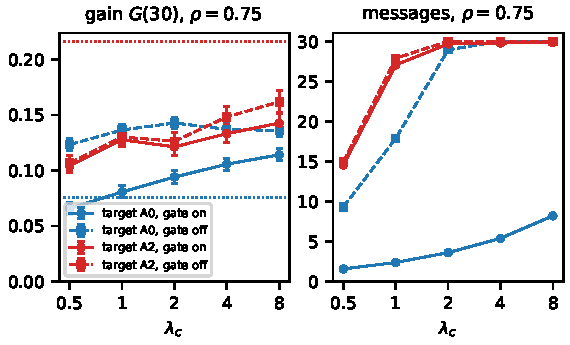
\includegraphics[width=0.62\linewidth]{figures/fig_rate.pdf}
\caption{Left: gain at $t = 30$ against the controller rate (target A0 blue, A2 red; gate on
solid, off dashed; dotted: Simulation 1 with one fact per night). Right: messages sent per
episode (budget 30). $\rho = 0.75$.}
\label{fig:rate}
\end{figure}

\begin{itemize}\itemsep1pt
\item \textbf{The rate changes the path more than the end point}
  (Figures~\ref{fig:gaintime}, \ref{fig:rate}). From $\lambda_c = 0.5$ to $8$ the gain at
  $t = 30$ rises from $0.10$ to $0.14$ (target A2) and from $0.07$ to $0.11$ (target A0).
\item \textbf{Fast controllers overshoot and relax}: a fast controller spends its budget within a
  few time units, its gain peaks early and then relaxes: target A2 at $\lambda_c = 8$ peaks at $0.26$
  ($t \approx 4.5$) and falls to $0.14$.
\item Because the A2 pool lies entirely on its target's side, more facts never hurt the false
  controller here (unlike in \texttt{task003-nosolution}).
\end{itemize}

\subsection{The vote gate and the proof stop}

The false controller is almost never stopped by the gate (the A2 share rarely reaches 75\%),
so turning the gate off changes nothing for it. The truth controller often is: with the gate
off it sends about six times as many messages (9.3 against 1.6 at $\lambda_c = 0.5$) and its
gain roughly doubles ($0.066 \to 0.123$; $+0.055$ at $\lambda_c = 1$, confirmed with fresh
draws). The proof stop has no effect larger than one agent's worth of belief ($1/24$) in any
setting, and turning it off costs up to 25 extra messages per episode.

\section{Who holds the proof}\label{sec:proof}

\begin{figure}[H]
\centering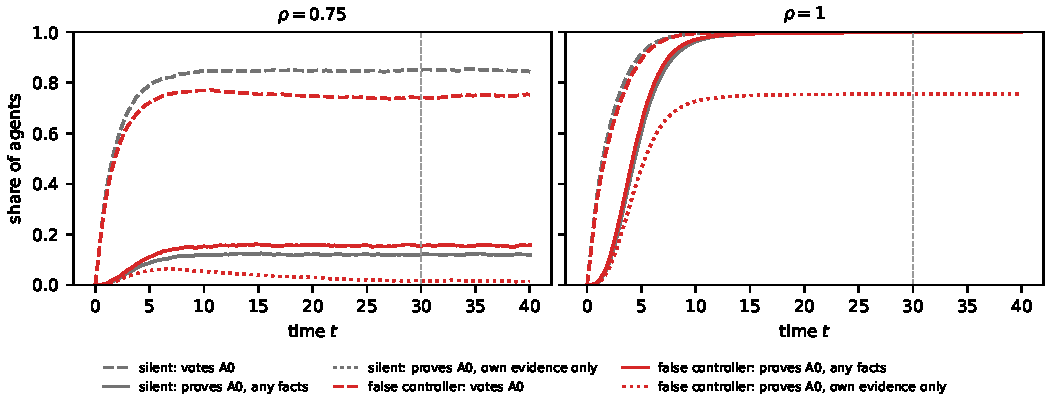
\includegraphics[width=0.95\linewidth]{figures/fig_proof_time.pdf}
\caption{Share of agents voting A0 (dashed), holding a proof of A0 from any facts they remember
(solid) and from their own original evidence only (dotted); silent (grey) against the false
controller (red). $q = 6$, $q_c = 12$, $\lambda_c = 1$, gate on.}
\label{fig:proof}
\end{figure}

\paragraph{Why memory decides.} With forgetting, a proof must be reassembled continually: at any
moment only 12\% of silent agents hold one (all from the agents' own facts). Under the false
controller about as many hold a proof (16\%), but almost none from their own evidence (2\%), and
the A0 vote falls to 74\%. With full memory every agent ends up proving A0, with or without a
controller, but under the false controller only 76\% do so from their own evidence: \textbf{the
controller's A2 facts are true}, so together with the agents' evidence they complete proofs of
A0. Every fact a truthful controller posts eventually narrows the possible worlds toward the real
one, and with full memory nothing is lost.

\paragraph{Help with the truth replaces the agents' own proofs.}

\begin{figure}[H]
\centering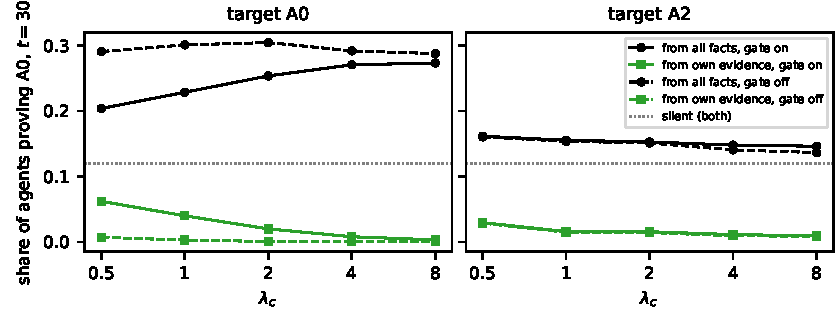
\includegraphics[width=0.66\linewidth]{figures/fig_own_proof.pdf}
\caption{Share of agents whose memory proves A0 at $t = 30$: from all their facts (black) and
from the agents' original facts only (green); dotted: silent swarm. $\rho = 0.75$.}
\label{fig:ownproof}
\end{figure}

Without a controller, 12\% of agents prove A0 at $t = 30$, all from the agents' own facts.
The truth controller raises the share proving A0 to 20--30\%, but the share proving it
\emph{from the agents' own facts} falls to 6\% (slow, gated controller) and to almost 0 when
it posts more (Figure~\ref{fig:ownproof}). Agents posting a controller fact do not post their
own, so their own evidence circulates less. The false controller, whose facts are also
true, raises proofs of A0 too (to 14--16\%) while own-evidence proofs fall to 1--3\%.
Simulation 1 shows the same substitution.

\section{The controller overestimates its support}

\begin{figure}[H]
\centering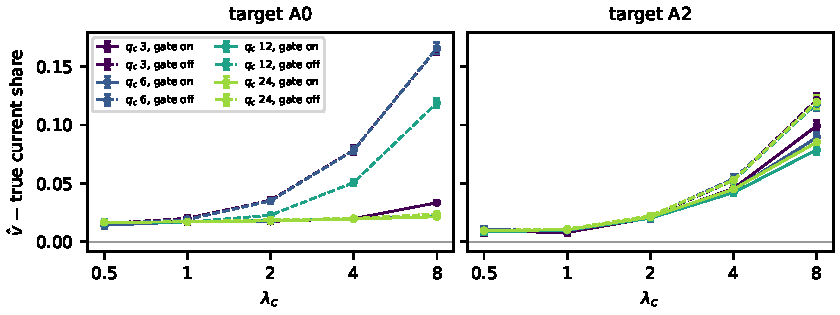
\includegraphics[width=0.66\linewidth]{figures/fig_sensing.pdf}
\caption{Error of the controller's estimate $\hat v$ (share of posts read whose author voted
for the target) against the true current share of all 24 agents' last votes; solid gate on,
dashed off.}
\label{fig:sensing}
\end{figure}

Unlike in Simulation 1, $\hat v$ is biased upward, and \textbf{the faster the controller, the
larger the bias}: about $+0.014$ at $\lambda_c \le 1$, rising to $+0.05$ (gate on) and $+0.14$
(gate off) at $\lambda_c = 8$. A likely reason, not yet tested: the posts it reads come from agents who
acted recently, often just after reading the controller's facts, while the true share also
counts older votes. More posts read ($q_c$) reduce the error's spread but not the bias.

%% ---------------------------------------------------------------------------------------------
\section{How readable is the command? Information and pair efficiency}\label{sec:eff}

A controller can change the swarm in two ways: in the direction it is asked to, or in ways that
happen whatever its target. We measure how readable the command is in the swarm (the mutual
information between the target and the swarm's state), which share of the change is directed (the
pair efficiency $\eta$), and how unsure the agents become. Throughout, the target is chosen by a fair
coin, and all quantities are taken at one time $t$, across the 1{,}000 episodes of each arm (not over
whole trajectories). Setting: $q = 6$. With full memory every agent proves A0 and nothing is
measurable, so only $\rho = 0.75$ is shown.

\subsection{Measures}

\begin{center}
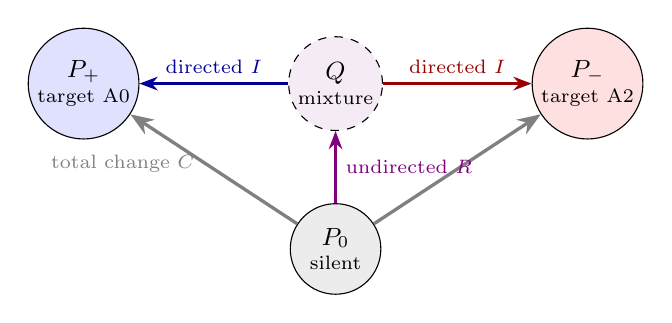
\begin{tikzpicture}[font=\small, dist/.style={draw, circle, minimum size=1.15cm, align=center, inner sep=1pt}]
  \node[dist, fill=gray!15] (P0) at (0,0) {$P_0$\\[-2pt]{\scriptsize silent}};
  \node[dist, fill=blue!12] (Pp) at (-3.2,2.1) {$P_+$\\[-2pt]{\scriptsize target A0}};
  \node[dist, fill=red!12] (Pm) at (3.2,2.1) {$P_-$\\[-2pt]{\scriptsize target A2}};
  \node[dist, dashed, fill=violet!8] (Q) at (0,2.1) {$Q$\\[-2pt]{\scriptsize mixture}};
  \draw[-{Stealth}, very thick, gray] (P0) -- node[left, font=\scriptsize, pos=0.55]{total change $C$} (Pp);
  \draw[-{Stealth}, very thick, gray] (P0) -- (Pm);
  \draw[-{Stealth}, thick, violet] (P0) -- node[right, font=\scriptsize]{undirected $R$} (Q);
  \draw[-{Stealth}, thick, blue!60!black] (Q) -- node[above, font=\scriptsize]{directed $I$} (Pp);
  \draw[-{Stealth}, thick, red!60!black] (Q) -- node[above, font=\scriptsize]{directed $I$} (Pm);
\end{tikzpicture}
\diagramcaption{Three distributions of the swarm's state at time $t$, one per arm, each over the
episodes of that arm. The controller's total change $C$ splits exactly into a part that depends on
its target ($I$, from the mixture $Q$ to each arm) and a part that does not ($R$, from silence to
$Q$). Efficiency $\eta = I/C$ is the directed share.}
\end{center}

\noindent\textbf{Distributions.} For each arm $a$ (silent $0$, target A0 $+$, target A2 $-$) and a
time $t$, each episode $e$ contributes a probability vector $y_a(e)$ over the values $x$ of the
state $X$: at \emph{one-agent} level its vote shares (the vote of a randomly chosen agent), at
\emph{swarm} level a mark on the bin of $s = m_{\text{A0}} - m_{\text{A2}}$ (difference of mean
beliefs, three equal bins on $[-1,1]$). Then $\hat P_a = \frac1n\sum_e y_a(e)$. Any pair of controllers
can be written as
\begin{equation}\label{eq:split}
\hat P_\pm = \hat P_0 + \mu \pm \delta,\qquad \mu = \tfrac12(\hat P_+ + \hat P_-) - \hat P_0,\quad
\delta = \tfrac12(\hat P_+ - \hat P_-),
\end{equation}
a \emph{common} part $\mu$ (what control does on average, whatever the target) and a
\emph{directional} part $\delta$; both are vectors over the values of $X$ (all answers, A1 included).

\noindent\textbf{Readability and the pair efficiency.} With $\hat Q = \hat P_0 + \mu$ and
$\mathrm{KL}(p\Vert q) = \sum_x p(x)\log_2[p(x)/q(x)]$,
\begin{equation}\label{eq:eta}
I = \tfrac12\mathrm{KL}(\hat P_+\Vert\hat Q) + \tfrac12\mathrm{KL}(\hat P_-\Vert\hat Q),\quad
C = \tfrac12\mathrm{KL}(\hat P_+\Vert\hat P_0) + \tfrac12\mathrm{KL}(\hat P_-\Vert\hat P_0) = I + R,\quad
R = \mathrm{KL}(\hat Q\Vert\hat P_0),\quad \eta = I/C .
\end{equation}
$I$ is the mutual information between the target and the state: how readable the command is
(at most 1 bit). With the one-agent state it is $I(\text{target};\text{vote of a randomly chosen
agent})$, the quantity mapped in Figure~\ref{fig:effI}. $I = \frac12\mathrm{KL}(\hat Q+\delta\Vert\hat Q) + \frac12\mathrm{KL}(\hat Q-\delta\Vert\hat Q)$
depends on $\delta$ and on where the pair sits ($\hat Q$); $R = \mathrm{KL}(\hat P_0+\mu\Vert\hat P_0)$ depends
only on $\mu$; $C$ (a number) $= I + R$, so $R = C - I$. The reference $\hat P_0$ is the silent arm. For
small changes, $\mathrm{KL}(p+\epsilon\Vert p) \approx \sum_x \epsilon(x)^2/(2\ln 2\,p(x))$ gives
\begin{equation}\label{eq:etasmall}
I \approx \frac{\Vert\delta\Vert^2}{2\ln 2},\quad R \approx \frac{\Vert\mu\Vert^2}{2\ln 2},\quad
\eta \approx \frac{1}{1 + \Vert \mu\Vert^2/\Vert\delta\Vert^2},\qquad \Vert v\Vert^2 = \sum_x \frac{v(x)^2}{\hat P_0(x)} .
\end{equation}
So $\eta = 1$ exactly when the two controllers' changes are mirror images ($\mu = 0$), whatever their
size, and $\eta$ falls only through the \emph{ratio} of common to directional change: when both push
the same way (a common push), or one moves the swarm much more than the other (a lopsided pair:
along one direction with sizes $a$ and $b$, $\Vert \mu\Vert/\Vert\delta\Vert = |a-b|/(a+b)$). It is a
property of the pair, not of either controller, and it stays constant whenever both effects grow
together; the size of the effect is measured by $I$. At swarm level $C$ is often infinite (the
controlled swarm reaches states silence never visits); there we use $\eta_{JS} = I/(I + \mathrm{JS}(\hat Q,\hat P_0))$ with the bounded
Jensen--Shannon divergence; $\mathrm{JS}(\hat Q,\hat P_0)$ is the information the state carries about
\emph{whether} a controller is present (controlled or silent, 50/50), so $\eta_{JS}$ compares
information about the direction with information about the presence of control.

\noindent\textbf{The agents' own uncertainty}: $\Delta\bar H$ (change in the mean entropy of their
beliefs) and $\Delta$JSD (change in disagreement, the entropy of the mean belief minus $\bar H$),
controlled minus silent, same episode.

\subsection{Over time}

\begin{figure}[!htb]
\centering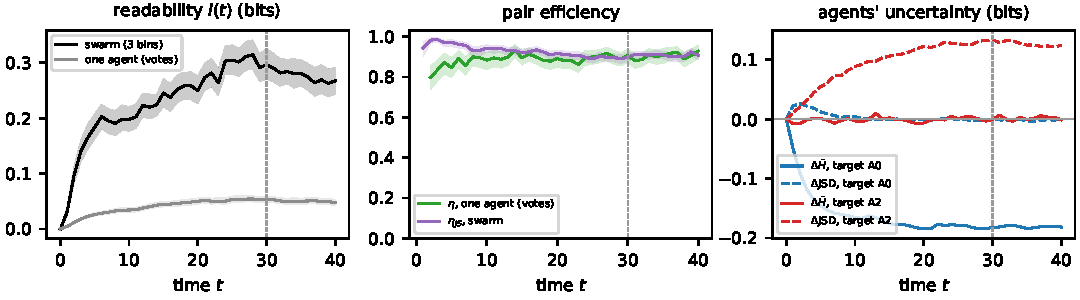
\includegraphics[width=0.92\linewidth]{figures/fig_eff_time2.pdf}
\caption{At $\rho = 0.75$, $q_c = 12$, $\lambda_c = 1$, gate on (the controller stops at $t = 30$,
dashed): readability $I(t)$ at swarm and one-agent level, pair efficiency ($\eta$, one agent;
$\eta_{JS}$, swarm), and the change in the agents' uncertainty. Bands: 95\% intervals over episodes.}
\label{fig:efftime2}
\end{figure}

\begin{figure}[!htb]
\centering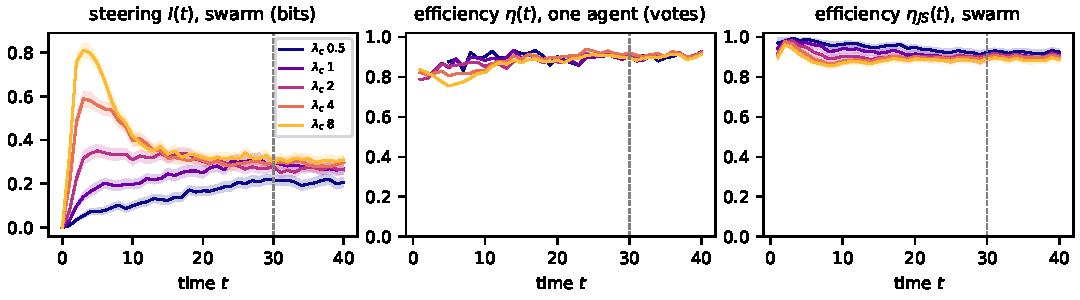
\includegraphics[width=0.66\linewidth]{figures/fig_eff_time.pdf}
\caption{Readability and pair efficiency over time, $\rho = 0.75$, $q_c = 12$, gate on, one line per
rate; the controller stops at $t = 30$ (dashed). Bands: 95\% intervals.}
\label{fig:efftime}
\end{figure}

\begin{itemize}\itemsep1pt
\item \textbf{Readability builds slowly and stays}: at $t = 30$, $I = 0.30$ bits (swarm) and
  $0.053$ bits (one agent's vote), $0.27$ and $0.048$ at $t = 40$. One agent's vote says little about
  the target, because most agents vote A0 whatever the controller.
\item \textbf{The pair is balanced} ($\eta = 0.91$, $\eta_{JS} = 0.90$).
\item \textbf{The false controller splits the swarm} ($\Delta$JSD $+0.13$) without changing individual
  certainty; the truth controller makes agents surer ($-0.18$ bits).
\end{itemize}

\subsection{Across the control plane}

\begin{figure}[!htb]
\centering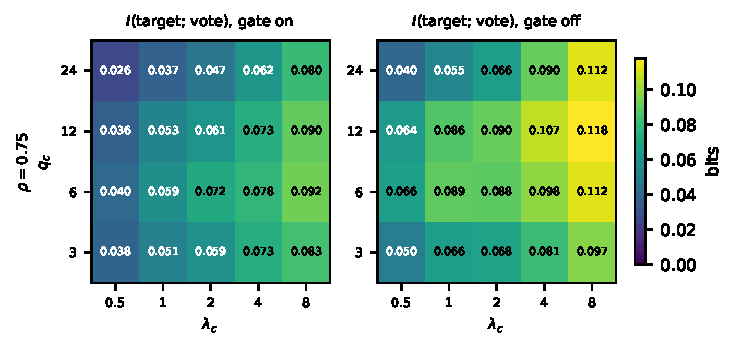
\includegraphics[width=0.6\linewidth]{figures/fig_eff_phase_I.pdf}
\caption{Readability $I(\text{target};\text{vote})$ at $t = 30$, in bits, over the reading budget $q_c$ (y)
and the controller rate $\lambda_c$ (x); state: the vote of a randomly chosen agent; $\rho = 0.75$.}
\label{fig:effI}
\end{figure}

\begin{figure}[!htb]
\centering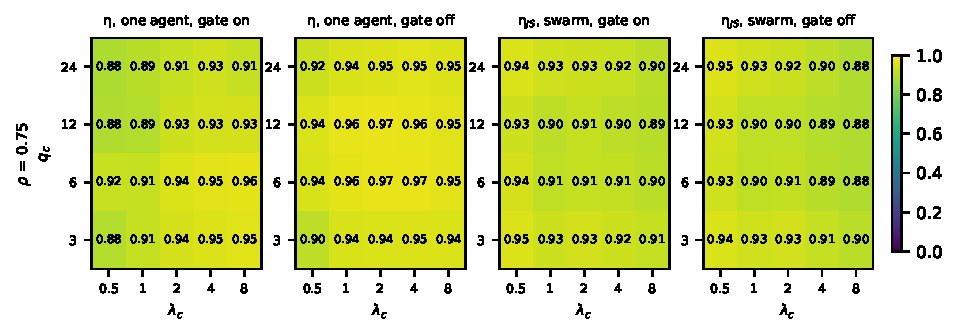
\includegraphics[width=0.55\linewidth]{figures/fig_eff_phase.pdf}
\caption{Pair efficiency at $t = 30$ over $q_c$ and the controller rate $\lambda_c$: one-agent $\eta$ (beliefs) and swarm
$\eta_{JS}$. Dash: undefined.}
\label{fig:effphase}
\end{figure}

\begin{itemize}\itemsep1pt
\item \textbf{Readability grows with the rate}: from 0.03--0.04 bits at $\lambda_c = 0.5$ to 0.08--0.09
  at $\lambda_c = 8$ with the gate on, and higher with the gate off (0.04--0.12), where the truth
  controller is no longer kept silent. It is lowest at $q_c = 24$ with the gate on: reading every
  post lets the gate silence the truth controller most often.
\item \textbf{$\eta$ is almost constant} (0.88--0.94; next subsection).
\end{itemize}

\subsection{Readability, pair efficiency and uncertainty against the controller rate}

\begin{figure}[!htb]
\centering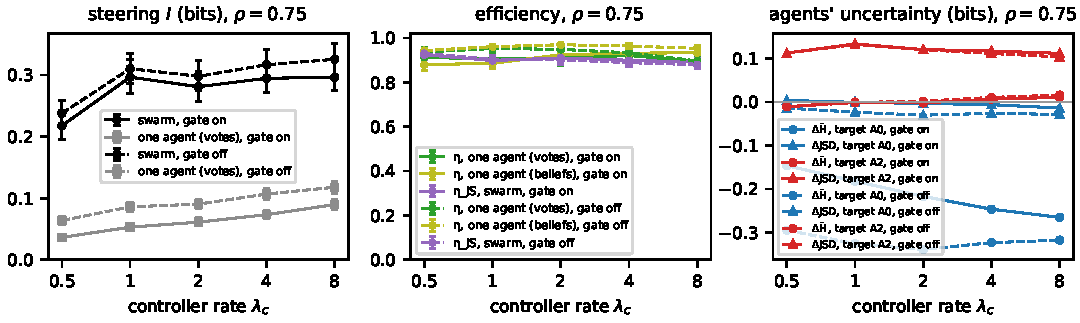
\includegraphics[width=0.72\linewidth]{figures/fig_eff_settings.pdf}
\caption{Readability $I$ (left), pair efficiency (middle) and the change in the agents' uncertainty
(right; circles $\Delta\bar H$, triangles $\Delta$JSD) at $t = 30$ against the controller rate $\lambda_c$ ($q_c = 12$; solid: gate on; dashed: gate off). Bars: 95\% intervals.}
\label{fig:effsettings}
\end{figure}

\begin{itemize}\itemsep1pt
\item \textbf{$\eta$ is almost constant (0.88--0.94) because every knob scales both controllers alike.}
  From $\lambda_c = 0.5$ (gate on) to $\lambda_c = 8$ (gate off) the A0 share moves $+0.07 / -0.09$ and then
  $+0.11 / -0.17$: both changes grow 1.7--2 times, $I$ and $R$ grow together, and by
  Eq.~(\ref{eq:etasmall}) their ratio, hence $\eta$, stays. In Simulation 1, larger batches make the
  false controller much stronger while the truth controller hits the ceiling, so $\eta$ falls.
\end{itemize}

\subsection{Precision at 50, 100 and 300 paths}

\begin{table}[H]
\centering\small
\caption{Value from 1{,}000 paths per arm, and root-mean-square error of the estimate from 50, 100
or 300 paths (200 random subsets each), at $t = 30$, $\lambda_c = 1$, $q_c = 12$, gate on, $\rho = 0.75$.}
\label{tab:effprec}
\begin{tabular}{lcccc}
\toprule
quantity & 1{,}000 paths & error, 50 & error, 100 & error, 300 \\
\midrule
steering $I$, swarm (3 bins) & 0.297 & 0.060 & 0.041 & 0.023 \\
steering $I$, one agent (votes) & 0.053 & 0.014 & 0.009 & 0.004 \\
efficiency $\eta$, one agent (votes) & 0.906 & 0.069 & 0.054 & 0.025 \\
efficiency $\eta_{JS}$, swarm & 0.899 & 0.047 & 0.032 & 0.015 \\
$\Delta\bar H$, target A0 & -0.182 & 0.029 & 0.019 & 0.010 \\
$\Delta\bar H$, target A2 & -0.000 & 0.023 & 0.015 & 0.008 \\
$\Delta$JSD, target A0 & -0.001 & 0.009 & 0.006 & 0.003 \\
$\Delta$JSD, target A2 & 0.133 & 0.012 & 0.008 & 0.004 \\
\bottomrule
\end{tabular}
\end{table}

\noindent Across all settings, at 100 paths: readability $\pm0.01$ (one agent) to $\pm0.03$ (swarm),
$\eta$ $\pm0.02$--$0.03$, $\Delta\bar H$ $\pm0.02$, $\Delta$JSD $\pm0.006$. Two settings that differ by
at least 0.02 are ordered correctly in 90--100\% of subsets.

%% ---------------------------------------------------------------------------------------------
\section{Success against facts posted}\label{sec:success}

The information measures above say how readable the command is, not whether the swarm ends up
deciding what the controller wants, nor at what cost. Here we measure both directly.

\begin{itemize}\itemsep1pt
\item \textbf{Collective decision} $Y_T$: plurality of the agents' last votes at time $T$; a tie
  between $k$ answers counts $1/k$. \textbf{Success}: $Y_T$ = the controller's target.
\item \textbf{Benefit} $\Delta_\pi = p_\pi - p_0$: change in the probability that the target wins,
  against the silent arm of the same episodes; $p_0$ is the silent probability.
\item \textbf{Cost} $C_\pi$: facts actually posted up to $T$, mean per run (not the allowed budget).
\item \textbf{Best-achievable curve} among the tested settings $\pi$ of one group ($\rho$, target):
  $\Delta^*(B) = \max\{\Delta_\pi : C_\pi \le B\}$, the largest gain reached spending at most $B$;
  read the other way, $C^*(\delta) = \min\{C_\pi : \Delta_\pi \ge \delta\}$, the least spending that
  reaches $\delta$. A setting below the curve is \emph{dominated}: another reached at least as much for less.
\item \textbf{Cost efficiency} $\eta_{\text{cost}} = C^*(\Delta_\pi)/C_\pi$: the share of the spending that
  was necessary (1: nothing cheaper reached as much). Not defined where $\Delta_\pi \le 0$ or its
  95\% interval includes 0.
\end{itemize}

\paragraph{How to read the curves.} Each dot is one setting, at (facts posted, gain). The
\textbf{solid line} is the best-achievable curve over the tested settings: it starts at $(0,0)$ (no
control) and steps up each time a setting reaches a higher gain than anything cheaper; dots on it have
$\eta_{\text{cost}} = 1$, dots below it are dominated, and $\eta_{\text{cost}}$ is how far to the left the
curve reaches the same gain. The \textbf{dashed line} is what becomes reachable if the controller
\emph{chooses its setting at random for each run}: using setting X (7 facts, $+0.32$) in half of the
runs and no control in the other half costs 3.5 facts and gains $+0.16$ \emph{on average}, so every
point on the straight segment between two settings (or between a setting and $(0,0)$) is reachable on
average; the dashed line is the outermost such segments (the concave hull through $(0,0)$). It lies above
the solid line where mixing beats every single setting. Its first segment from $(0,0)$ is arithmetic,
not an observation.

\begin{center}
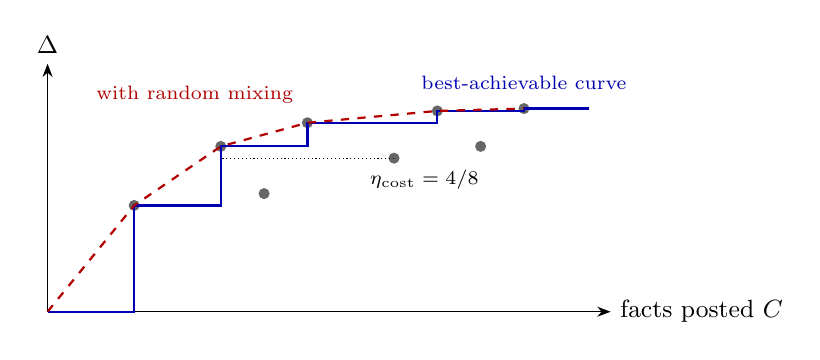
\begin{tikzpicture}[font=\small, x=0.55cm, y=3cm]
  \draw[-{Stealth}] (0,0) -- (13,0) node[right]{facts posted $C$};
  \draw[-{Stealth}] (0,0) -- (0,1.05) node[above]{$\Delta$};
  \foreach \c/\d in {2/0.45, 4/0.7, 6/0.8, 9/0.85, 11/0.86, 5/0.5, 8/0.65, 10/0.7}
     \fill[black!60] (\c,\d) circle (2pt);
  \draw[thick, blue!70!black] (0,0) -- (2,0) -- (2,0.45) -- (4,0.45) -- (4,0.7) -- (6,0.7) -- (6,0.8) -- (9,0.8) -- (9,0.85) -- (11,0.85) -- (11,0.86) -- (12.5,0.86);
  \draw[thick, dashed, red!70!black] (0,0) -- (2,0.45) -- (4,0.7) -- (6,0.8) -- (9,0.85) -- (11,0.86);
  \draw[densely dotted] (8,0.65) -- (4,0.65);
  \node[font=\scriptsize, align=left] at (8.7,0.56) {$\eta_{\text{cost}} = 4/8$};
  \node[font=\scriptsize, blue!70!black] at (11,0.97) {best-achievable curve};
  \node[font=\scriptsize, red!70!black] at (3.4,0.92) {with random mixing};
\end{tikzpicture}
\diagramcaption{Illustration. Each point is a setting. Solid: best-achievable curve; dashed: reachable
on average by random mixing per run. The setting at cost 8 reaches $\Delta = 0.65$, which a setting
costing 4 already reaches: $\eta_{\text{cost}} = 0.5$.}
\end{center}

\begin{figure}[H]
\centering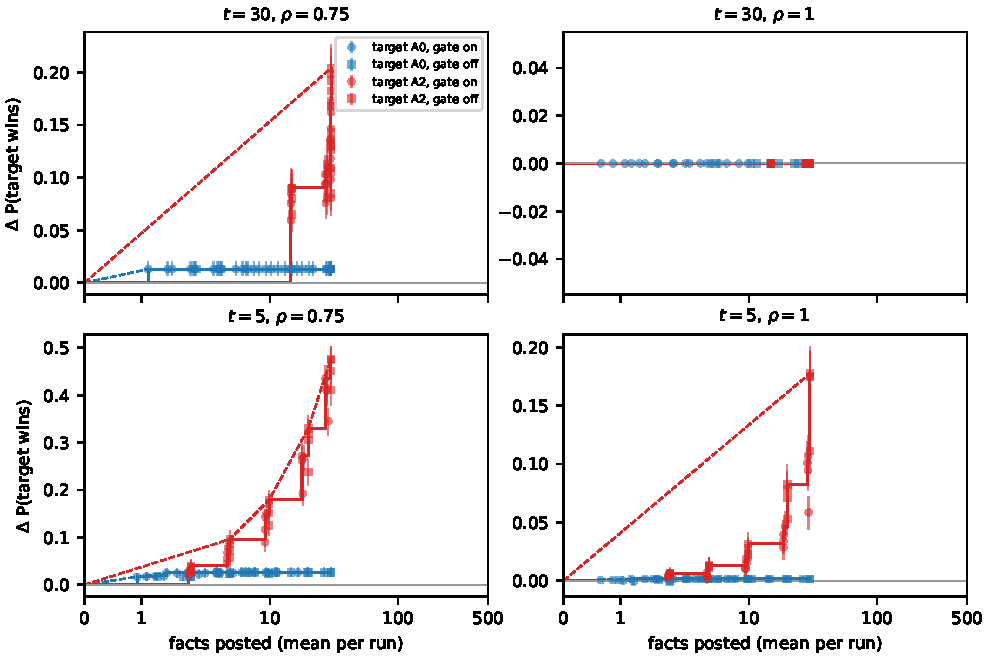
\includegraphics[width=0.84\linewidth]{figures/fig_success_facts.pdf}
\caption{Change in the probability that the controller's target wins against facts posted, at
$t = 30$ (top) and $t = 5$ (bottom), $\rho = 0.75$ (left) and $1$ (right); every setting
($q_c \times \lambda_c \times$ gate, $q = 6$, proof stop on) with its 95\% interval; blue: target A0,
red: target A2; circles gate on, squares gate off. Solid: best-achievable curve; dashed: with random
mixing per run. The x axis is linear from 0 to 1 and logarithmic above, up to 500 as in Simulation 1.}
\label{fig:success}
\end{figure}

\begin{itemize}\itemsep1pt
\item \textbf{The truth controller has no room}: without control A0 already wins 98.7\% of runs when
  agents forget (100\% with full memory), so its gain is at most $+0.013$ (blue dots near 0).
\item \textbf{Overturning the proof has increasing returns.} At $t = 30$, when agents forget, the
  false controller raises the chance that A2 wins by $+0.06$ to $+0.20$ for 14.6 to 30 facts, and the
  gain is still rising at the 30-message cap. The dashed line lies above the solid one: to raise the
  chance by $0.1$, the best single setting needs 27 facts, while using a strong setting in half of the
  runs and no control in the other half needs 15 on average. Concentrated control pays; the tested
  settings (a steady rate) do not include it.
\item \textbf{Here $\eta_{\text{cost}}$ cannot rank the settings}: when the gain keeps growing with
  cost, most settings are the best at their own cost (15 of 40 on the curve, median
  $\eta_{\text{cost}}$ 0.99). That means ``no clear waste'', not ``efficient''.
\item \textbf{With full memory the false controller wins only early}: at $t = 5$ it raises the chance
  that A2 wins by up to $+0.18$ (fast, gate off); by $t = 30$ the gain is 0. When agents forget, the
  $t = 5$ gain reaches $+0.48$ (fast, gate off) before relaxing to $+0.20$ (Section~\ref{sec:strength}).
\item \textbf{Precision at 100 paths}: $\Delta$ $\pm0.017$; $\eta_{\text{cost}}$ $\pm0.02$--$0.035$.
\end{itemize}

\paragraph{Caveats.} One world (task\_003), 24 agents, exact-Bayesian agents,
probability-matching votes; a controller without memory that posts one fact at a time; a
budget of 30 messages. Means over 1{,}000 episodes per setting. Efficiencies are relative to the
tested settings. Full analysis, code and tables:
\texttt{analysis/task003\_llm\_free/simulation\_2/analysis/} (report of 9 October, reviewer guide)
and \texttt{analysis/task003\_llm\_free/efficiency\_estimates/}.

\end{document}
